\documentclass[a4paper]{article}
\usepackage{amsmath,amsfonts,amsthm,amssymb}
\usepackage{graphicx}

\begin{document}
\section*{The Question}
The \emph{exterior angle bisector theorem} states that if \(\frac{DB}{DA}=\frac{CB}{CA}\) holds for a point \(D\) on \(AB\) produced, then \(DC\) bisects \(\angle ECB\),
where \(E\) lies on \(AC\) produced. By constructing a suitable line parallel to \(DC\) or otherwise, prove this theorem.
\section*{Solution}
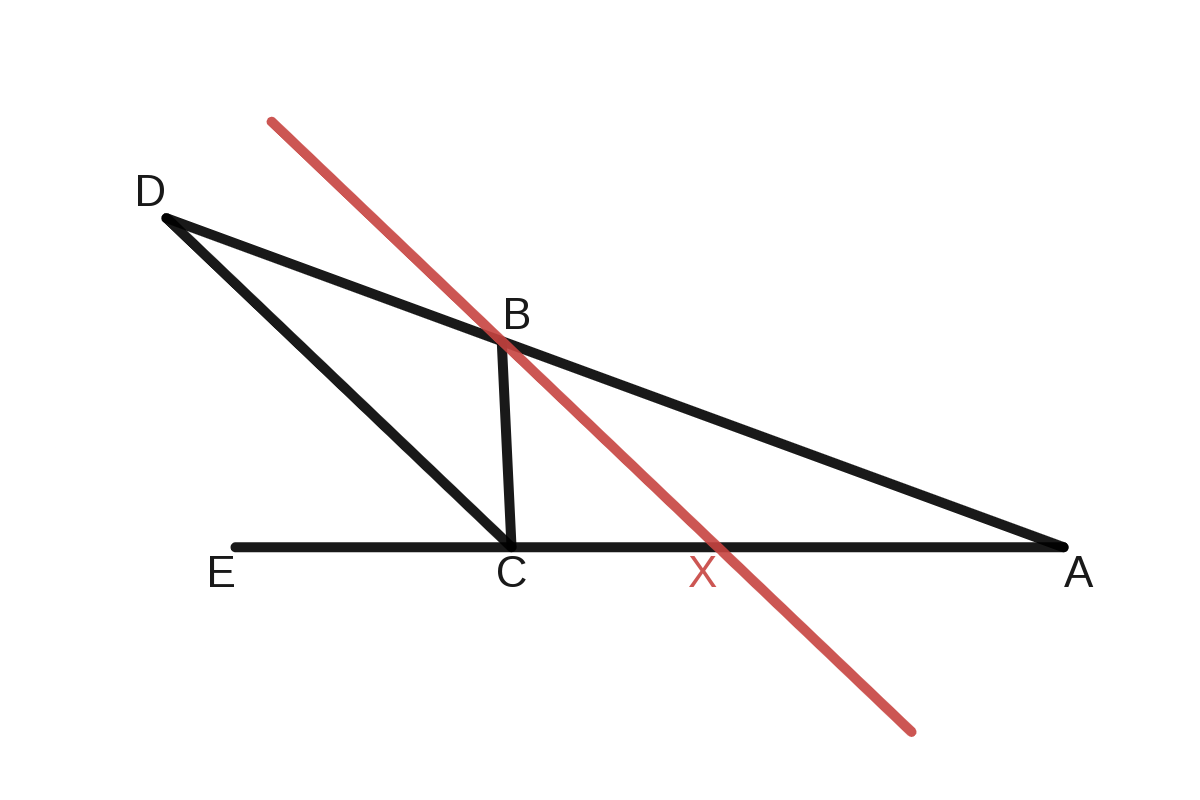
\includegraphics[width=\textwidth]{dreaded.png}
By mid-point theorem, since \(DC\parallel BX\), \(\frac{DB}{DA}=\frac{CX}{CA}\). It is given that \(\frac{DB}{DA}=\frac{CB}{CA}\). Hence, \(\frac{CX}{CA}=\frac{DB}{DA}=\frac{CB}{CA}\iff CX=CB\). Since \(\triangle CXB\) is isosceles, \(\angle CXB=\angle BXC\). Let them be \(\theta\). By angular sum of \(\triangle CXB\), \(\angle BCX=\pi-2\theta\).
By corresponding angles, since \(DC\parallel BX\), \(\angle DCE=\theta\). By adjacent angles on a straight line, \(\angle DCB=\pi-\theta-(\pi-2\theta)=\theta=\angle DCE\).\qed
\end{document}
